\section{Background}\label{sec:background}
The use of LIBS technology in planetary exploration has proven to be effective in analyzing soil and rock samples \citep{knight2000}.

A laser pulses to ablate and remove any surface contaminants, such as dust and weathering layers, to expose the underlying material.
The laser generates a plasma plume from the now-exposed sample material.
This plasma plume emits light, which, when collected and analyzed, reveals the elemental composition of the sample by correlating the intensity of emitted light with specific wavelengths in a LIBS spectrum.
The LIBS technique enables remote analysis of materials without the need for sample preparation.
It allows for rapid analysis because of the immediate spectrum collection from the subsequent plasma, while maintaining a high spatial resolution due to its small observation footprints.
This high resolution is essential for pinpointing and investigating small features. \cite{wiensChemcam2012}

% In 2013, \citet{wiensPreFlight3} published a paper describing the pre-flight calibration and initial data processing for the ChemCam LIBS instrument.
% This paper introduces methods for preprocessing spectra samples and a regression model based on Partial Least Squares (PLS2) used to predict the composition of geological samples on Mars.
% The model was trained on a dataset of 69 rock samples from Earth, which were created in a laboratory to simulate the conditions of the Martian surface.
% This dataset is referred to as the calibration dataset.
% Two key conclusions were drawn from this paper:
% \begin{enumerate}
%     \item A larger dataset is needed to improve the accuracy of the model.
%     \item The PLS2 model is not ideal for this type of data, and an argument is made for using PLS1 instead because of its ability to optimize each element separately, which in can improve the accuracy although it suffers slower run times.
% \end{enumerate}

% Based on this work, \citet{cleggRecalibrationMarsScience2017} published a paper in 2017 describing a new approach to the ChemCam LIBS calibration model.
% This paper introduces a new model based on PLS1 with a sub-model approach (PLS-SM) and Independent Component Analysis (ICA).
% In addition, a much larger calibration dataset was used, consisting of 408 samples.
% Using this, the team was able to improve the predictions by employing a \textit{submodel} PLS approach in tandem with ICA.
% This model is referred to as the Multivariate Oxide Composition (MOC) model.
% The MOC model is currently used by the ChemCam team to analyze the LIBS data collected by the Curiosity rover.

% MULTICOLINEARITY & MATRIX EFFECTS - EXPLANATION
% Multicollinearity: In computational terms, multicollinearity represents a challenge for feature selection and model interpretability. Traditional regression algorithms struggle when variables (features) are highly correlated because they cannot easily isolate the contribution of each variable to the prediction (output). This hampers the model's ability to generalize well to new data and makes it difficult to understand which features are most important for the prediction task. Advanced techniques like ridge regression or feature extraction methods may be required to handle this.
%
% Matrix Effects: These constitute a challenge in data preprocessing and normalization. In machine learning terms, matrix effects introduce a form of 'class imbalance' or 'data skew.' The model can be misled by the dominant features (in this case, spectral lines influenced by matrix effects) and fail to generalize well. Dealing with this requires sophisticated preprocessing techniques or specialized algorithms capable of handling imbalanced or skewed data.

% MULTICOLINEARITY & MATRIX EFFECTS - PROSE
% However, the interpretation of LIBS data poses significant computational challenges.
% First, a high degree of multicollinearity exists within the spectral data, rendering traditional linear analysis methods less effective.
% The multicollinearity arises due to the correlation among different spectral channels, influenced both by the multi-line emission characteristics of individual elements and by geochemical correlations between elements.
% Secondly, the complexity of LIBS spectra is increased by multiple interacting physical processes.
% These interactions, collectively referred to as 'matrix effects,' introduce variability into the emission line intensities independent of the elements' concentrations.
% Such variability complicates the direct interpretation of the spectra and poses challenges for computational models aiming for accurate elemental quantification.\cite{andersonImprovedAccuracyQuantitative2017}


\subsection{The Multivariate Oxide Composition Model}\label{sec:moc}
\begin{figure}[H]
    \centering
    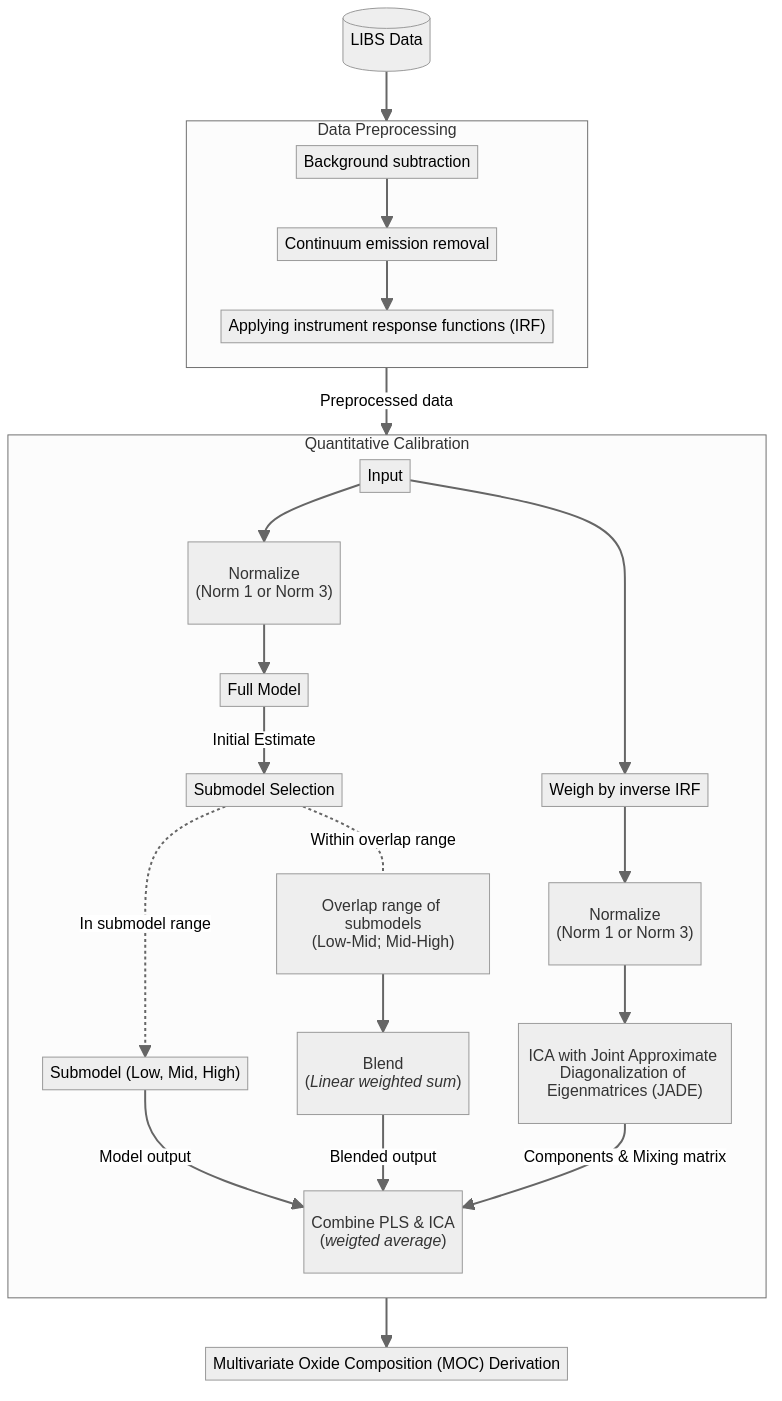
\includegraphics[width=0.45\textwidth]{images/pipeline.png}
    \caption{Flowchart illustrating the data processing and calibration steps for Laser-Induced Breakdown Spectroscopy (LIBS) data leading to the derivation of Multivariate Oxide Composition (MOC).}
    \label{fig:libs_data_processing}
\end{figure}

We illustrate the data processing and calibration steps for LIBS data leading to the derivation of Multivariate Oxide Composition (MOC) in Figure \ref{fig:libs_data_processing}. The MOC model is described in details by \citet{cleggRecalibrationMarsScience2017} and \citet{andersonImprovedAccuracyQuantitative2017}, but we provide a brief overview here, which will serve as a foundation for the subsequent discussion of our work.

\subsection{Data Preprocessing}\label{sec:data_preprocessing}

The initial phase of processing the raw emission data records (EDR) involves a series of steps to clean up the spectra for subsequent analysis.
The pipeline, as illustrated in Figure \ref{fig:libs_data_processing}, commences with the subtraction of the dark spectrum.
This step is crucial to isolate the signal emanating solely from the plasma, thereby removing the effects of ambient light and reflected sunlight that are present when the laser is not employed.

To further refine the spectra, an undecimated wavelet transform is applied.
This advanced signal processing technique effectively reduces noise while preserving the essential features of the spectrum.
The subsequent wavelength calibration ensures the precise alignment of spectra by compensating for wavelength shifts as a function of temperature across every pixel.

A critical step in preprocessing is the removal of the continuum, which predominantly arises from Bremsstrahlung emission and ion recombination.
The continuum is subtracted because it carries minimal information pertinent to the target material's composition.
The processed data, at this stage, is referred to as the reduced data record (RDR).

The final step in data preparation involves the conversion of the spectral data from counts to photons by applying an instrument response function (IRF) correction.
This yields a set of cleaned and calibrated spectra (CCS), primed for the subsequent compositional analysis.

\subsection{Multivariate Oxide Composition Derivation}\label{sec:moc_derivation}

The multivariate analysis employs a composite approach integrating partial least squares regression with submodels (PLS-SM) and independent component analysis (ICA) to derive the Multivariate Oxide Composition (MOC).
The PLS-SM approach utilizes tailored sub-models for distinct composition ranges, enhancing accuracy at the boundaries of these ranges.
Independent Component Analysis assists in distinguishing elemental emission lines, contributing to a refined multivariate model.

Two normalization methods are employed in the analysis: Norm 1 and Norm 3.
Norm 1 standardizes the full spectrum across all three spectrometers such that the sum total is unity.
In contrast, Norm 3 conducts normalization on a per-spectrometer basis, culminating in a full normalized spectrum summing to three.
The optimal normalization technique is selected based on its efficacy in model performance for the specific analysis task at hand.

\subsubsection{Outlier Removal}\label{sec:outlier_removal}

In their analysis, \citet{andersonImprovedAccuracyQuantitative2017} employed a methodical outlier removal process to enhance model accuracy in multivariate regression. To detect outliers, they utilized influence plots, leveraging statistical measures that reflect each data point's deviation from the model's predictions and their influence on the model due to their position in the predictor space.

The process involves using influence plots, which display points by their spectral residual, or $Q$ statistic, and leverage, $h_{T}$. Leverage is computed as $h_{t} = \text{diag}\left[ t(t^{T}t)^{-1}t^{T} \right]$, reflecting the distance of an observation's predictors from those of other observations. High leverage points are prospective outliers with respect to independent variables. The relationship between leverage and Hotelling's $T^{2}$ statistic indicates that leverage can serve as a measure of spectral distance from the center of space defined by the latent variables of the model.
The residual $Q$ is a metric of fit, quantifying the sum of the squared differences between the observed spectrum $X$ and the model-reconstructed spectrum using scores $t$ and loadings $P$, with $e = X - tP'$ and $Q_{i} = e_{i}e_{i}'$. By marking each spectrum from the training dataset on an influence plot with coordinates based on leverage and residual $Q$, outliers stand out distinctly from the cloud of points either along the leverage, residual, or both axes.

Outlier removal is performed iteratively; an initial PLS model is conceived with cross-validation to determine the optimum number of latent variables, followed by an inspection of the influence plot to pinpoint outliers. Identified outliers are excised, and the model is re-run. This procedure is repeated as needed, ensuring that any removals do not degrade the model's general performance. The presence of 'masking' further necessitates multiple iterations, where the excision of some outliers may reveal others previously obscured.


\subsubsection{Partial Least Squares Sub-Models}\label{sec:pls_submodels}

\citet{andersonImprovedAccuracyQuantitative2017} proposed an approach referred to as the Partial Least Squares Sub-Models (PLS1-SM).
The inherent variability of LIBS spectral responses to different element concentrations necessitates a nuanced analysis. High element concentrations tend to obscure the spectral signal, and the presence of other elements further complicates the spectral response. A single regression model typically falls short in accounting for such variations, leading to compromises in predictive precision for specific samples.

They deployed multiple regression models, each tailored to subsets of the entire composition range, targeting "low," "mid," and "high" concentrations along with a comprehensive "full model." This led to the formation of 32 distinct models, with selected sub-model ranges that prioritize both a robust dataset and precise compositional response.

Each sub-model was subjected to training, cross-validation, and optimization phases, which included the iterative outlier removal strategy mentioned in section~\ref{sec:outlier_removal}. The full model's preliminary composition estimation of unknown targets dictates the choice of subsequent sub-model(s) for refined prediction.

PLS1-SM blends predictions from sub-models with overlapping concentration ranges. The predictions are linearly combined for a cohesive prediction. The full model projection $y_{\text{full}}$, if within a blend-ready range, determines the final prediction $y_{\text{final}}$ through a weighted sum of overlapping sub-model predictions:

\begin{align*}
w_{\text{mid}} &= \frac{y_{\text{full}}-y_{\text{blend range, min}}}{y_{\text{blend range, max}} - y_{\text{blend range, min}}} \\
w_{\text{low}} &= 1 - w_{\text{mid}} \\
y_{\text{final}} &= w_{\text{low}}\cdot y_{\text{low}} + w_{\text{mid}}\cdot y_{\text{mid}} 
\end{align*}

This applies analogously for predictions in the "mid-high" range to prevent prediction discontinuities.

The exact delineations of the blending ranges are adjustable, with optimization performed using the Broyden-Fletcher-Goldfarb-Shannon (BFGS) algorithm. This process, aimed at minimizing the RMSE for the full model dataset, established optimal ranges. Initial blend boundaries were predicated on sub-model intersections, with exceptional outliers managed distinctly due to their deviation from expected value ranges.

\subsubsection{Independent Component Analysis}\label{sec:ica}
\citet{cleggRecalibrationMarsScience2017} and \cite{forniIndependentComponentAnalysis2013} proposed the use of Independent Component Analysis (ICA) to identify the elemental emission lines in LIBS spectra. Independent Component Analysis (ICA) is a computational method used to separate a multivariate signal into additive, statistically independent components, particularly useful in scenarios where the signal sources overlap, such as in Laser-Induced Breakdown Spectroscopy (LIBS).

ICA yields independent source components and the affiliated mixing matrix which illustrates how the independent sources are combined to form the observed spectral data.

After the extraction of independent components, the key task is to associate each independent component with a single elemental emission line. This involves examining the elements' emission lines and determining the ICA scores, which are then utilized to derive a calibration curve relating the ICA score to the composition.

To ascertain the accuracy of this calibration, a regression analysis is performed using multiple regression functions. The function that provides the most reliable fit (often assessed through chi-square values) is used to predict the composition for each element.

Model refinement is facilitated by techniques such as normalization, outlier removal (via Median Absolute Deviation), and k-fold cross-validation. These methods ensure the robustness and reliability of the predictive model constructed through ICA.

In summary, the detailed pipeline for LIBS data processing and analysis integrates a comprehensive suite of preprocessing, multivariate analysis, and optimization techniques, as delineated in the process flow of Figure \ref{fig:libs_data_processing}.
The harmonized use of PLS-SM, ICA, and meticulous outlier management culminates in a robust method for quantifying the oxide composition of the studied materials.